\documentclass[11pt]{article}
\usepackage[a4paper,margin=1in]{geometry}
\usepackage{amsmath,amssymb,amsthm,mathtools}
\usepackage{algorithm}
\usepackage{algpseudocode}
\usepackage{tikz}
\usetikzlibrary{arrows.meta,positioning,calc,fit,backgrounds}
\usepackage{booktabs}
\usepackage{microtype}
\usepackage{enumitem}
\usepackage{hyperref}
\usepackage{xcolor}
\usepackage{caption}
\usepackage{float}
\usepackage{cleveref}
\setlength{\parindent}{0pt}
\setlength{\parskip}{0.55em}
\hypersetup{colorlinks=true,linkcolor=black,citecolor=black,urlcolor=blue}

\newtheorem{lemma}{Lemma}
\newtheorem{theorem}{Theorem}
\newtheorem{proposition}{Proposition}
\newtheorem{remark}{Remark}

\newcommand{\Sset}{\mathcal{S}_t}
\newcommand{\Uset}{\mathcal{U}_t}
\newcommand{\Fset}{\mathcal{F}_t}
\newcommand{\Iset}{\mathcal{I}_t}
\newcommand{\PathU}{\mathcal{P}(\mathcal{U}_t)}
\newcommand{\dist}{\delta}

\title{\textbf{Dijkstra Is NOT Greedy: A Global-to-Local Proof of Correctness}}
\author{Shengbao Wang\\\small Hangzhou Normal University}
\date{}

\begin{document}
\maketitle
\vspace{-2.5em}

\begin{abstract}
Dijkstra's algorithm is traditionally classified as a greedy algorithm. This paper argues that this classification misrepresents the mechanism by which the algorithm determines shortest paths. We present a direct global-to-local proof of correctness. At each iteration, the algorithm identifies a shortest path over the entire set of paths whose endpoints remain unsolved. This global minimum is necessarily a shortest path to its own endpoint. More fundamentally, the algorithm uses already determined shortest paths to establish one additional shortest path at each iteration. We identify this progression as dynamic programming. A three-step exclusion proof shows how the full path space is reduced to frontier candidates, how relaxation removes inferior alternatives, and why minimum extraction yields the global minimum. The choice is thus determined by a global comparison, not by an optimistic local greedy choice. We conclude that the algorithm is more accurately characterized by dynamic programming and deterministic path exclusion than by the traditional greedy classification.
\end{abstract}

\section{Introduction}
Since Dijkstra introduced it in 1959 \cite{Dijkstra1959}, this elegant shortest-path algorithm has become one of the best-known algorithms in computer science. It has important practical applications, including route planning in map navigation and routing in communication networks \cite{SedgewickWayne2011}. It has also long been regarded as a standard greedy algorithm. This classification is prominent in classical textbooks \cite{BrassardBratley1988,KleinbergTardos2006,CLRS2022}. Kleinberg and Tardos describe greedy decisions as being made \emph{myopically}, with each step optimizing a local criterion. Cormen et al. characterize Dijkstra as greedy because it selects the unsettled vertex with the smallest tentative distance. Their correctness proof then establishes the finality of the selected vertex's distance. Sedgewick and Wayne present the same minimum-distance and relaxation operations, while Princeton course materials likewise place shortest paths among greedy algorithms \cite{SedgewickWayne2011,WayneCOS423}. Roughgarden offers a particularly clear example: a minimum boundary candidate is selected, and its optimality for the chosen endpoint is subsequently proved \cite{Roughgarden2018}.

These proofs are rigorous. They also employ properties of paths that cross the boundary of the settled set. Their principal conclusion, however, concerns the shortest-path distance of the \emph{selected endpoint}. The choice is stated before its correctness is established. This order supports the customary picture of a local greedy decision followed by a proof of its safety. It does not expose the stronger fact that the selected candidate is the minimum over \emph{all paths to currently unsolved destinations}.

The dynamic-programming character of shortest-path algorithms has also been studied. Bellman's principle of optimality and Lawler's treatment provide important foundations \cite{Bellman1957,Lawler1976}. Sniedovich analyzes Dijkstra as a dynamic-programming procedure, while Misra gives a fixed-point interpretation \cite{Sniedovich2006,Misra2001}. Lew examines the relationship between greedy algorithms and dynamic programming, but still describes Dijkstra as greedy \cite{Lew2006}. These studies reveal important recursive features. They do not make the global minimization over all unsolved-destination paths the central object of the correctness argument.

This paper takes that global path space as its starting point. We prove that every iteration identifies its absolute shortest path. The shortest path to the selected endpoint then follows directly from this global result. To establish this claim, we give a three-step exclusion proof. The first step restricts the search to the frontier. The second uses optimal substructure and relaxation to retain the best candidate for each frontier vertex. The third determines the minimum over the remaining candidates. These reductions correspond to the operations of Dijkstra's algorithm itself.

The resulting interpretation reverses the familiar explanatory order. The algorithm does not reach a global conclusion by trusting a locally attractive choice. Instead, deterministic exclusions establish the global minimum before its endpoint is declared solved. Each iteration uses previously established shortest paths to obtain a new one. We therefore argue that Dijkstra's algorithm is fundamentally a dynamic-programming algorithm, and that its customary classification as greedy is incorrect. This claim concerns the mathematical basis of its minimum selection, not the validity of earlier correctness proofs.

\section{Preliminaries and the Search-Space Partition}
\label{sec:prelim}
Let $G=(V,E,w)$ be a finite directed weighted graph with source $s\in V$. To make the exclusion argument especially transparent, we assume strictly positive edge weights throughout:
\[
  w(e)>0\qquad (e\in E).
\]
For a path $P$, let $w(P)$ be the sum of its edge weights. Write $\delta(s,v)$ for the shortest-path distance to a vertex $v$ reachable from $s$. Vertices not reachable from $s$ are not included in the finite-distance minimizations below; if no unsolved vertex is reachable, the procedure terminates.

\subsection{A motivating first step}
The source $s$ itself may be regarded as the first solved vertex, at distance $0$. The next vertex to be solved is particularly easy to identify: it is an endpoint of a minimum-weight outgoing edge from $s$. Indeed, putting
\[
  m=\min_{(s,v)\in E}w(s,v),
\]
any such one-edge path has length $m$. Every path from $s$ with two or more edges must start with an outgoing edge whose length is at least $m$ and must then add at least one positive-weight edge. Thus every multi-edge path is strictly longer than $m$. The minimum-weight one-edge path is the absolute shortest among all nonempty paths starting at $s$.

The underlying observation is elementary: \emph{adding an edge to a path necessarily makes it longer}. It also prompts the question driving this paper. Does every subsequent iteration likewise identify an absolute shortest path from a global set of paths that are still relevant? Our proof answers yes.

\subsection{Dijkstra's original three-way partition}
Dijkstra already divided vertices into three classes in Problem 2 of his original paper \cite{Dijkstra1959}. Set A contains vertices with known shortest paths. Set B contains the remaining vertices directly connected to A; the next vertex is chosen from this set. Set C contains all other vertices. We use different symbols but retain this three-region structure.

At iteration $t$, let $\Sset$ be the \emph{solved set}, for which
\[
 d(x)=\delta(s,x)\qquad (x\in\Sset),
\]
and let $\Uset=V\setminus\Sset$ be the \emph{unsolved set}. The initially solved set is $\{s\}$, with $d(s)=0$. Within $\Uset$, define
\[
\Fset=\{f\in\Uset:\exists x\in\Sset\text{ such that }(x,f)\in E\}
\]
as the \emph{frontier} and $\Iset=\Uset\setminus\Fset$ as the \emph{invisible set}. These are disjoint partitions:
\[
 V=\Sset\;\dot\cup\;\Uset,
 \qquad \Uset=\Fset\;\dot\cup\;\Iset.
\]
Here ``invisible'' means only that the vertex is not directly exposed by an outgoing edge from the current solved set. Figure~\ref{fig:spatial} illustrates Dijkstra's original three-region partition in our notation. For directed graphs, the frontier uses edges directed \emph{out of} the solved region.

\begin{figure}[H]
\centering
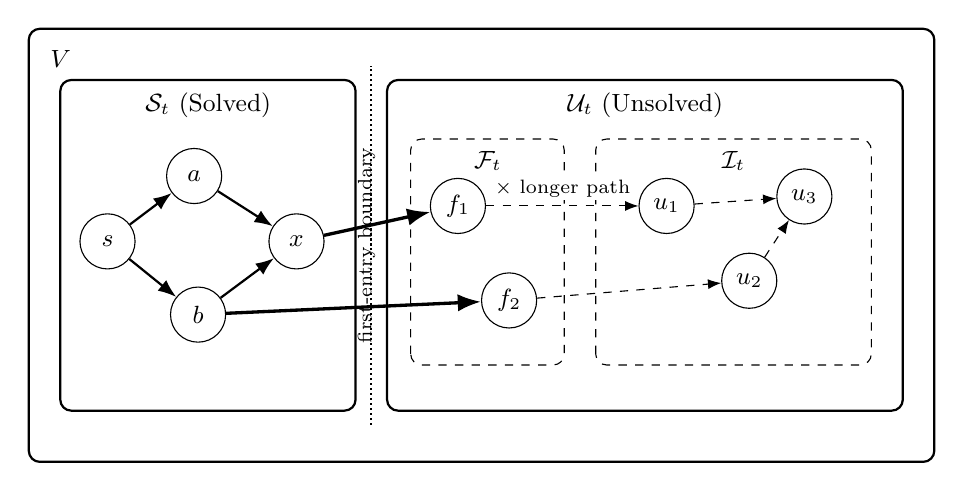
\begin{tikzpicture}[
    >=Latex,
    vertex/.style={circle,draw,minimum size=7mm,inner sep=1pt},
    every node/.style={font=\small}
]
% Entire vertex space
\draw[thick,rounded corners] (-0.4,-2.75) rectangle (11.1,2.75);
\node[anchor=north west] at (-0.25,2.60) {$V$};

% Solved / unsolved containers
\draw[thick,rounded corners] (0.0,-2.10) rectangle (3.75,2.10);
\node at (1.88,1.78) {$\mathcal{S}_t$ (Solved)};

\draw[thick,rounded corners] (4.15,-2.10) rectangle (10.70,2.10);
\node at (7.43,1.78) {$\mathcal{U}_t$ (Unsolved)};

% Frontier and invisible partitions
\draw[dashed,rounded corners] (4.45,-1.52) rectangle (6.40,1.35);
\node at (5.43,1.07) {$\mathcal{F}_t$};

\draw[dashed,rounded corners] (6.80,-1.52) rectangle (10.30,1.35);
\node at (8.55,1.07) {$\mathcal{I}_t$};

% Solved vertices
\node[vertex] (s) at (0.60,0.05) {$s$};
\node[vertex] (a) at (1.70,0.88) {$a$};
\node[vertex] (b) at (1.75,-0.88) {$b$};
\node[vertex] (x) at (3.00,0.05) {$x$};

\draw[->,thick] (s) -- (a);
\draw[->,thick] (a) -- (x);
\draw[->,thick] (s) -- (b);
\draw[->,thick] (b) -- (x);

% Frontier vertices and boundary-crossing edges
\node[vertex] (f1) at (5.05,0.50) {$f_1$};
\node[vertex] (f2) at (5.70,-0.70) {$f_2$};
\draw[->,very thick] (x) -- (f1);
\draw[->,very thick] (b) -- (f2);

% Invisible vertices and deeper continuations
\node[vertex] (u1) at (7.70,0.50) {$u_1$};
\node[vertex] (u2) at (8.75,-0.45) {$u_2$};
\node[vertex] (u3) at (9.45,0.62) {$u_3$};
\draw[->,dashed] (f1) -- (u1);
\draw[->,dashed] (u1) -- (u3);
\draw[->,dashed] (f2) -- (u2);
\draw[->,dashed] (u2) -- (u3);

% Mark a continuation beyond the first unsolved vertex as excluded in Step 1
\node[font=\scriptsize,fill=white,inner sep=1pt] at (6.38,0.72) {$\times$ longer path};

% First-entry boundary
\draw[densely dotted,thick] (3.95,-2.28) -- (3.95,2.28);
\node[rotate=90,font=\scriptsize] at (3.89,0) {first-entry boundary};

% Bottom labels
\end{tikzpicture}
\caption{Dijkstra's three-way partition at iteration $t$, in our notation. Every path from $s$ to an unsolved vertex first enters the frontier $\mathcal{F}_t$. With positive edge weights, any further extension is longer than this first-entry prefix.}
\label{fig:spatial}
\end{figure}

\subsection{The first-entry property}
The partition has a simple but decisive consequence.

\begin{lemma}[First-entry lemma]\label{lem:firstentry}
Let $P=(v_0=s,v_1,\ldots,v_k=u)$ be any path ending at $u\in\Uset$. If $v_j$ is the first vertex of $P$ in $\Uset$, then $v_{j-1}\in\Sset$ and $v_j\in\Fset$.
\end{lemma}
\begin{proof}
By the choice of $j$, all preceding vertices of $P$, in particular $v_{j-1}$, belong to $\Sset$. Since $(v_{j-1},v_j)\in E$ and $v_j\in\Uset$, the definition of $\Fset$ gives $v_j\in\Fset$.
\end{proof}

Thus every path from the source into the unsolved region first reaches a frontier vertex. Even a path ending deep in $\Iset$ cannot bypass this boundary. This fact will justify the first exclusion in Section~\ref{sec:proof}.

\section{The Global-to-Local Principle and Path Exclusion}
\label{sec:principle}
\subsection{The global path space}
For each $u\in\Uset$, let $\mathcal P(s,u)$ be the set of paths from $s$ to $u$. Define the global search space at iteration $t$ by
\[
  \PathU=\bigcup_{u\in\Uset}\mathcal P(s,u).
\]
The objective of the iteration is to identify
\[
  P_t^*\in\arg\min_{P\in\PathU}w(P).
\]
The minimum is taken over \emph{all paths ending at unsolved vertices}, not over a collection of shortest paths that are assumed to have already been found.

\subsection{From a global minimum to a local shortest path}
Suppose $P_t^*$ ends at $u^*$. Since
\[
  \mathcal P(s,u^*)\subseteq\PathU,
\]
every path $Q$ from $s$ to $u^*$ satisfies
\[
  w(P_t^*)\le w(Q).
\]
Thus a path that minimizes the global search space necessarily minimizes the path set for its own endpoint. \emph{One global shortest path therefore settles one additional vertex.} The remaining task is to show how Dijkstra determines this global minimum without enumerating all paths.

\subsection{The exclusion principle}
To find the shortest path, one may exclude any path that is strictly longer than another admissible candidate. Indeed, if $P_1$ is admissible and $w(P_1)<w(P_2)$, then $P_2$ cannot attain the current minimum. If several candidates tie, retaining one is sufficient to determine a shortest path.

This exclusion refers to the \emph{current iteration}. A path extended beyond the first unsolved vertex may be irrelevant to the present global minimum, but its later edges can become relevant after that vertex is settled. The three-step proof below uses this distinction to reduce the current search space without losing any future shortest-path solution.

\section{A Three-Step Exclusion Proof of Correctness}
\label{sec:proof}
Fix iteration $t$ with a nonempty reachable frontier. Distances $d(x)=\delta(s,x)$ for all $x\in\Sset$ are already finalized. We prove that Dijkstra's next extraction realizes the global minimum in $\PathU$.

\subsection{Step 1: Frontier exclusion}
Take an arbitrary path
\[
  P=(s=v_0,v_1,\ldots,v_k=u)\in\PathU.
\]
Let $v_j$ be its first unsolved vertex. By Lemma~\ref{lem:firstentry}, $v_j\in\Fset$. Its prefix $P^{\mathrm{first}}=(v_0,\ldots,v_j)$ also belongs to $\PathU$. If $P$ continues past $v_j$, it must acquire at least one more positive-weight edge, so
\[
  w(P^{\mathrm{first}})<w(P).
\]
Thus no path containing more than one unsolved vertex can be the current global minimum: a shorter path already ends at its first frontier vertex. What remains relevant at this iteration is the form
\[
  s\rightsquigarrow x\to f,
  \qquad x\in\Sset,\quad f\in\Fset,
\]
with every internal vertex in the solved set and exactly one unsolved vertex, its endpoint $f$. This is the mathematical reason why it suffices to consider frontier vertices rather than paths going further into the unsolved region.

\subsection{Step 2: Relaxation exclusion}
Fix $f\in\Fset$. Every candidate surviving Step 1 is of the form
\[
  P=Q(s,x)\circ(x,f),\qquad x\in\Sset.
\]
First consider the prefix to $x$. Since $x$ has already been solved, an arbitrary prefix $Q(s,x)$ cannot improve on $d(x)=\delta(s,x)$. If it is strictly longer, replacing it by a finalized shortest prefix produces a strictly shorter candidate to $f$. We therefore need only the candidate value
\[
  d(x)+w(x,f)
\]
for each boundary edge $(x,f)$. This is the optimal-substructure reason why relaxation extends finalized shortest distances, rather than enumerating earlier paths.

Several solved predecessors may lead to the same frontier vertex $f$. The shortest candidate among them is
\[
  D_t(f)=
  \min_{\substack{x\in\Sset\\(x,f)\in E}}
  \{d(x)+w(x,f)\}.
\]
All longer candidates to this same endpoint can now be excluded; if candidates tie, one representative suffices. Thus Step 2 comprises both optimal-prefix replacement and same-endpoint minimization. Both reductions are reflected in the relaxation operation. After Step 2, the current search is represented by the frontier values
\[
  \{D_t(f):f\in\Fset\}.
\]

\subsection{Step 3: Global minimum extraction}
Choose
\[
 f^*\in\arg\min_{f\in\Fset}D_t(f),
 \qquad D^*=D_t(f^*).
\]
We show that this is the minimum not only among frontier representatives but among \emph{all} paths in $\PathU$.

Take any $P\in\PathU$. Let $f$ be its first unsolved vertex, $x$ its predecessor, and $L_x$ the length of the prefix from $s$ to $x$. As $x\in\Sset$, $d(x)\le L_x$. Since $D_t(f)$ is the least candidate over all solved-to-$f$ boundary edges,
\[
 D_t(f)\le d(x)+w(x,f)\le L_x+w(x,f).
\]
The remainder of $P$ after $f$ has nonnegative length, so $w(P)\ge L_x+w(x,f)$. By the choice of $f^*$, $D_t(f)\ge D_t(f^*)$. Combining gives
\[
 \begin{aligned}
 w(P)&\ge L_x+w(x,f)\\
     &\ge d(x)+w(x,f)\\
     &\ge D_t(f)\\
     &\ge D_t(f^*)=D^*.
 \end{aligned}
\]
A path attaining $D^*$ exists, namely an already finalized shortest prefix followed by the corresponding boundary edge. Therefore
\[
  D^*=\min_{P\in\PathU} w(P).
\]

\begin{theorem}[Correctness of one iteration]\label{thm:iteration}
If all edge weights are positive and at least one unsolved vertex is reachable, then any $f^*$ minimizing $D_t(f)$ over $\Fset$ satisfies
\[
  D_t(f^*)=\delta(s,f^*).
\]
Hence its shortest-path distance can be finalized.
\end{theorem}
\begin{proof}
By the preceding inequalities, a path attaining $D_t(f^*)$ is globally shortest in $\PathU$. In particular, it is shortest among the paths to its own endpoint $f^*$, which form a subset of $\PathU$.
\end{proof}

The solved state then grows and the unsolved endpoint set shrinks:
\[
 \mathcal S_{t+1}=\Sset\cup\{f^*\},\qquad
 \mathcal U_{t+1}=\Uset\setminus\{f^*\}.
\]
The same reasoning applies at the next iteration.

\subsection{Correspondence with the standard algorithm}
\label{sec:correspondence}
The three exclusions are not additional operations. They account for the operations already performed by the standard algorithm, as summarized in Table~\ref{tab:correspondence}. Frontier restriction implements Step 1; relaxation maintains the reduced candidate values of Step 2; and \textsc{Extract-Min} implements Step 3.

\begin{table}[htbp]
\centering
\caption{Exclusion steps and corresponding operations in Dijkstra's algorithm.}
\label{tab:correspondence}
\small
\begin{tabular}{@{}p{0.24\linewidth}p{0.29\linewidth}p{0.39\linewidth}@{}}
\toprule
Exclusion step & Standard operation & Mathematical role \\
\midrule
Step 1: Frontier exclusion & Frontier restriction & Omit paths that continue beyond their first unsolved vertex. \\
Step 2: Relaxation exclusion & Relaxation of tentative distances & Use optimal solved prefixes and retain the best candidate for each frontier endpoint. \\
Step 3: Global minimum & \textsc{Extract-Min} & Select the global minimum among the surviving candidates. \\
\bottomrule
\end{tabular}
\end{table}

To make the correspondence between the three-step exclusion proof and the original algorithm more explicit, Algorithm~\ref{alg:standard} presents a compact version of Dijkstra's procedure, with the relevant operations annotated. It starts with the source $s$ in the solved set and immediately relaxes its outgoing edges. The first minimum extraction therefore uses frontier values that have already been computed. In later iterations, the relaxations following an extraction update the frontier values for the next extraction. Hence, although the loop places \textsc{Extract-Min} before relaxation, the state used by each extraction already reflects Step~2. Step~1 is implicit in that state: an unsolved vertex not yet exposed by the solved set has distance label $\infty$, so it cannot be chosen while a reachable frontier candidate remains.

\begin{algorithm}[htbp]
\caption{Dijkstra's algorithm with the source settled initially}\label{alg:standard}
\begin{algorithmic}[1]
\State $d(s)\gets 0$; $d(v)\gets\infty$ for $v\ne s$
\State $\mathcal S\gets\{s\}$; $Q\gets V\setminus\{s\}$ (queue keyed by $d$)
\For{each $(s,v)\in E$ with $v\in Q$}
  \State $d(v)\gets\min\{d(v),w(s,v)\}$; update $v$'s key in $Q$ \Comment{Step 2: initial relaxation}
\EndFor
\While{$Q\ne\varnothing$}
  \State $u\gets\operatorname{ExtractMin}(Q)$ \Comment{Step 3: frontier minimum}
  \If{$d(u)=\infty$} \State \textbf{break} \EndIf
  \State $\mathcal S\gets\mathcal S\cup\{u\}$
  \For{each $(u,v)\in E$ with $v\in Q$}
    \If{$d(u)+w(u,v)<d(v)$}
      \State $d(v)\gets d(u)+w(u,v)$; update $v$'s key in $Q$ \Comment{Step 2: relaxation}
    \EndIf
  \EndFor
\EndWhile
\end{algorithmic}
\end{algorithm}

Dijkstra's original account already uses three vertex classes and a sequence of candidate updates followed by minimum selection \cite{Dijkstra1959}. The present proof identifies the global path-minimization argument behind that established process. It is a proof of the original algorithm, not a modified algorithm.

\section{Discussion: Dynamic Programming Rather Than Greedy Selection}
\label{sec:discussion}
\subsection{The dynamic-programming recurrence}
The recursive structure follows directly from Step 2. For each frontier vertex $f$,
\[
 D_t(f)=\min_{\substack{x\in\Sset\\(x,f)\in E}}
 \{d(x)+w(x,f)\}.
\]
All distances $d(x)$ on the right are final. The global frontier minimum establishes one more final distance, which is then available in later iterations. In this way, the set of solved shortest paths grows through repeated applications of optimal substructure. The finalized distances form a nondecreasing sequence, as successive iterations minimize over progressively smaller sets of unsolved destinations.

The recurrence can be compared with the familiar Fibonacci computation,
\[
 F_0=0,\qquad F_1=1,\qquad F_n=F_{n-1}+F_{n-2}.
\]
Both procedures construct a new exact result from previously solved subproblems. Their dependency structures differ. The next Fibonacci index is fixed in advance. In Dijkstra, the next vertex is determined by the current frontier and its weights. Nevertheless, neither computation requires guessing the value of the next solved subproblem. This common incremental structure supports the dynamic-programming interpretation of Dijkstra.

\subsection{Why the greedy classification is incorrect}
The standard greedy account emphasizes the immediate minimum-distance selection. The usual meaning of this account is a decision based on the best available local criterion, without first examining all possible future continuations. Kleinberg and Tardos explicitly describe the stepwise rule of a greedy algorithm as \emph{myopic} \cite{KleinbergTardos2006}. Such a description may suggest an optimistic local choice whose success has to be established afterward.

The textbook correctness argument commonly follows that order: select the minimum tentative label, then prove that its value is final for the selected vertex. These proofs are mathematically valid, and they use comparisons with paths crossing the settled boundary. Yet their stated target is the optimality of that particular endpoint. They do not begin by minimizing over the union of \emph{all} paths ending at unsolved vertices. The global-to-local proof makes that stronger minimization the starting point of the argument.

Our three exclusions establish, before finalizing the next vertex, that no path in the current global space is shorter than the chosen boundary candidate. The minimum is therefore not an optimistic, short-sighted, or blind local guess. It is a consequence of a complete and directed elimination of inferior paths. Moreover, the procedure relies on shortest paths already obtained and uses them to determine a new shortest path. We accordingly reject the greedy classification and identify dynamic programming as the more accurate account of Dijkstra's algorithm. Its minimum-extraction operation is the final expression of deterministic global exclusion, not the origin of the algorithm's correctness.

\section{Conclusion}
This paper has given a global-to-local proof of Dijkstra's algorithm. Three deterministic exclusions reduce the paths to unsolved destinations to frontier candidates, then to one optimal candidate per frontier vertex, and finally to the global shortest path. Its endpoint's shortest-path optimality follows directly from that global minimum.

Each iteration uses previously established shortest paths to determine one new shortest path. This is a dynamic-programming process, not a speculative local greedy choice. The result places Dijkstra alongside Bellman--Ford and Floyd--Warshall, which are already widely understood as dynamic-programming shortest-path algorithms \cite{CLRS2022}. It thus provides a more unified conceptual classification of these major classical shortest-path algorithms.

\section*{Acknowledgments}
The author thanks Zimo Wang for helpful discussions that made the central ideas of this work clearer. The author also acknowledges the assistance of AI large language models, specifically Gemini and ChatGPT, in drafting, translation, and editorial refinement of the manuscript.

\begin{thebibliography}{99}

\bibitem{Dijkstra1959}
E.~W. Dijkstra,
``A note on two problems in connexion with graphs,''
\emph{Numerische Mathematik}, vol.~1, pp.~269--271, 1959.
doi:10.1007/BF01386390.

\bibitem{SedgewickWayne2011}
R. Sedgewick and K. Wayne,
\emph{Algorithms}, 4th ed.
Upper Saddle River, NJ: Addison-Wesley Professional, 2011.

\bibitem{BrassardBratley1988}
G. Brassard and P. Bratley,
\emph{Algorithmics: Theory and Practice}.
Englewood Cliffs, NJ: Prentice Hall, 1988.

\bibitem{KleinbergTardos2006}
J. Kleinberg and E. Tardos,
\emph{Algorithm Design}.
Boston, MA: Pearson/Addison-Wesley, 2006.

\bibitem{CLRS2022}
T.~H. Cormen, C.~E. Leiserson, R.~L. Rivest, and C. Stein,
\emph{Introduction to Algorithms}, 4th ed.
Cambridge, MA: MIT Press, 2022.

\bibitem{WayneCOS423}
K. Wayne,
``COS 423: Analysis of Algorithms---Greedy Algorithms: Shortest Path,''
Princeton University, course materials.
[Online]. Available: \url{https://www.cs.princeton.edu/~wayne/cs423/}.

\bibitem{Roughgarden2018}
T. Roughgarden,
\emph{Algorithms Illuminated, Part 2: Graph Algorithms and Data Structures}.
San Francisco, CA: Soundlikeyourself Publishing, LLC, 2018.

\bibitem{Bellman1957}
R. Bellman,
\emph{Dynamic Programming}.
Princeton, NJ: Princeton University Press, 1957.

\bibitem{Lawler1976}
E.~L. Lawler,
\emph{Combinatorial Optimization: Networks and Matroids}.
New York, NY: Holt, Rinehart and Winston, 1976.

\bibitem{Sniedovich2006}
M. Sniedovich,
``Dijkstra's algorithm revisited: The dynamic programming connexion,''
\emph{Control and Cybernetics}, vol.~35, no.~3, pp.~599--620, 2006.

\bibitem{Misra2001}
J. Misra,
``A walk over the shortest path: Dijkstra's algorithm viewed as fixed-point computation,''
\emph{Information Processing Letters}, vol.~77, nos.~2--4, pp.~197--200, 2001.
doi:10.1016/S0020-0190(00)00202-7.

\bibitem{Lew2006}
A. Lew,
``Canonical greedy algorithms and dynamic programming,''
\emph{Control and Cybernetics}, vol.~35, no.~3, pp.~621--643, 2006.

\end{thebibliography}

\end{document}
